\documentclass[crop=false]{standalone}
%\documentclass{standalone}
\usepackage{tikz} % To generate the plot from csv
\usepackage{pgfplots}
\usepackage{graphicx}
\usepackage{booktabs}
\usepackage{subfig}
\usepackage{float}
\usepackage[section]{placeins} % getting figures below sections
\usepackage{blindtext}
\usepackage{siunitx}
\usepgfplotslibrary{units} % Allows to enter the units nicely
\usetikzlibrary{external} %https://tex.stackexchange.com/questions/1460/script-to-automate-externalizing-tikz-graphics
\tikzexternalize[prefix=savedfigures/]

\pgfplotsset{compat=newest} % Allows to place the legend below plot
\usepackage{pgfplotstable}
\usepgfplotslibrary{statistics}

% #################### Function definition for box plots read table ##################\
\makeatletter
\pgfplotsset{
	boxplot prepared from table/.code={
		\def\tikz@plot@handler{\pgfplotsplothandlerboxplotprepared}%
		\pgfplotsset{
			/pgfplots/boxplot prepared from table/.cd,
			#1,
		}
	},
	/pgfplots/boxplot prepared from table/.cd,
	table/.code={\pgfplotstablecopy{#1}\to\boxplot@datatable},
	row/.initial=0,
	make style readable from table/.style={
		#1/.code={
			\pgfplotstablegetelem{\pgfkeysvalueof{/pgfplots/boxplot prepared from table/row}}{##1}\of\boxplot@datatable
			\pgfplotsset{boxplot/#1/.expand once={\pgfplotsretval}}
		}
	},
	make style readable from table=lower whisker,
	make style readable from table=upper whisker,
	make style readable from table=lower quartile,
	make style readable from table=upper quartile,
	make style readable from table=median,
	make style readable from table=average,
	make style readable from table=lower notch,
	make style readable from table=upper notch
}
\makeatother
\begin{document}

\section{23 1 Mandl6 SA Mutations AMALGAM 20210814 233100}

% ######################## UTRP SA Mutation operators applied ######################## 
\begin{figure} 
\centering 
\tikzsetnextfilename{UTRP_DBMOSA_BP_mutation_funcs_Best_comp} 
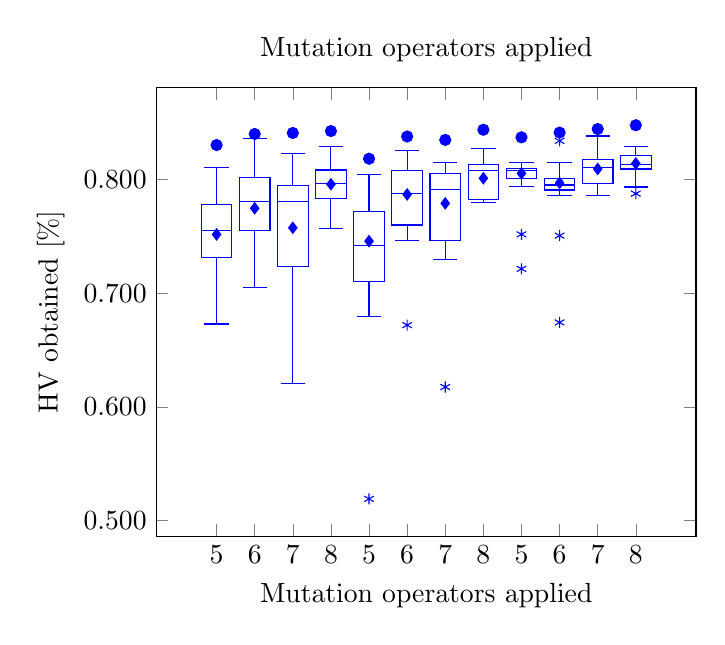
\begin{tikzpicture} 
\begin{axis}[ 
title={Mutation operators applied}, 
boxplot/draw direction=y, 
xtick={1,2,3,4,5,6,7,8,9,10,11,12}, 
xticklabels={5,6,7,8,5,6,7,8,5,6,7,8}, 
x tick label style={rotate=0, align=center}, 
xlabel={Mutation operators applied}, 
y tick label style={/pgf/number format/.cd,fixed,precision=3, zerofill}, 
ylabel={HV obtained [\%]}, 
] 

% ############## B_Mutations_AMALGAM=5 ################## 
\addplot[boxplot, mark=asterisk, 
boxplot prepared={ 
lower whisker=0.67291, 
upper whisker=0.81022, 
lower quartile=0.73129, 
upper quartile=0.7778, 
median=0.75542, 
average=0.7516}, 
color = blue, solid, area legend] 
coordinates {}; 
\addplot[only marks,mark=*,color = blue]coordinates{(1,0.83023)}; 

% ############## B_Mutations_AMALGAM=6 ################## 
\addplot[boxplot, mark=asterisk, 
boxplot prepared={ 
lower whisker=0.70515, 
upper whisker=0.83585, 
lower quartile=0.7549, 
upper quartile=0.80185, 
median=0.7805, 
average=0.77464}, 
color = blue, solid, area legend] 
coordinates {}; 
\addplot[only marks,mark=*,color = blue]coordinates{(2,0.83995)}; 

% ############## B_Mutations_AMALGAM=7 ################## 
\addplot[boxplot, mark=asterisk, 
boxplot prepared={ 
lower whisker=0.6204, 
upper whisker=0.82258, 
lower quartile=0.72359, 
upper quartile=0.79503, 
median=0.78095, 
average=0.75746}, 
color = blue, solid, area legend] 
coordinates {}; 
\addplot[only marks,mark=*,color = blue]coordinates{(3,0.84084)}; 

% ############## B_Mutations_AMALGAM=8 ################## 
\addplot[boxplot, mark=asterisk, 
boxplot prepared={ 
lower whisker=0.75692, 
upper whisker=0.82871, 
lower quartile=0.7835, 
upper quartile=0.80831, 
median=0.79656, 
average=0.79577}, 
color = blue, solid, area legend] 
coordinates {}; 
\addplot[only marks,mark=*,color = blue]coordinates{(4,0.84252)}; 

% ############## B_Mutations_AMALGAM_every_n=5 ################## 
\addplot[boxplot, mark=asterisk, 
boxplot prepared={ 
lower whisker=0.67956, 
upper whisker=0.80459, 
lower quartile=0.70988, 
upper quartile=0.77144, 
median=0.74179, 
average=0.74573}, 
color = blue, solid, area legend] 
coordinates {
(5,0.51917)}; 
\addplot[only marks,mark=*,color = blue]coordinates{(5,0.81819)}; 

% ############## B_Mutations_AMALGAM_every_n=6 ################## 
\addplot[boxplot, mark=asterisk, 
boxplot prepared={ 
lower whisker=0.74649, 
upper whisker=0.82563, 
lower quartile=0.75992, 
upper quartile=0.80781, 
median=0.78768, 
average=0.78674}, 
color = blue, solid, area legend] 
coordinates {
(6,0.67189)}; 
\addplot[only marks,mark=*,color = blue]coordinates{(6,0.83773)}; 

% ############## B_Mutations_AMALGAM_every_n=7 ################## 
\addplot[boxplot, mark=asterisk, 
boxplot prepared={ 
lower whisker=0.72969, 
upper whisker=0.81491, 
lower quartile=0.74656, 
upper quartile=0.80519, 
median=0.79102, 
average=0.77898}, 
color = blue, solid, area legend] 
coordinates {
(7,0.61748)}; 
\addplot[only marks,mark=*,color = blue]coordinates{(7,0.83474)}; 

% ############## B_Mutations_AMALGAM_every_n=8 ################## 
\addplot[boxplot, mark=asterisk, 
boxplot prepared={ 
lower whisker=0.77947, 
upper whisker=0.82736, 
lower quartile=0.78228, 
upper quartile=0.81334, 
median=0.80771, 
average=0.80101}, 
color = blue, solid, area legend] 
coordinates {}; 
\addplot[only marks,mark=*,color = blue]coordinates{(8,0.84368)}; 

% ############## B_Mutations_Counts_normal=5 ################## 
\addplot[boxplot, mark=asterisk, 
boxplot prepared={ 
lower whisker=0.7941, 
upper whisker=0.81461, 
lower quartile=0.80094, 
upper quartile=0.80974, 
median=0.80745, 
average=0.80531}, 
color = blue, solid, area legend] 
coordinates {
(9,0.72137)
(9,0.75171)}; 
\addplot[only marks,mark=*,color = blue]coordinates{(9,0.83698)}; 

% ############## B_Mutations_Counts_normal=6 ################## 
\addplot[boxplot, mark=asterisk, 
boxplot prepared={ 
lower whisker=0.78568, 
upper whisker=0.81487, 
lower quartile=0.79065, 
upper quartile=0.80073, 
median=0.79513, 
average=0.79692}, 
color = blue, solid, area legend] 
coordinates {
(10,0.75058)
(10,0.83387)
(10,0.67426)}; 
\addplot[only marks,mark=*,color = blue]coordinates{(10,0.84115)}; 

% ############## B_Mutations_Counts_normal=7 ################## 
\addplot[boxplot, mark=asterisk, 
boxplot prepared={ 
lower whisker=0.78547, 
upper whisker=0.83815, 
lower quartile=0.79673, 
upper quartile=0.81736, 
median=0.81022, 
average=0.8092}, 
color = blue, solid, area legend] 
coordinates {}; 
\addplot[only marks,mark=*,color = blue]coordinates{(11,0.84429)}; 

% ############## B_Mutations_Counts_normal=8 ################## 
\addplot[boxplot, mark=asterisk, 
boxplot prepared={ 
lower whisker=0.79334, 
upper whisker=0.82857, 
lower quartile=0.80917, 
upper quartile=0.82112, 
median=0.8132, 
average=0.81402}, 
color = blue, solid, area legend] 
coordinates {
(12,0.7875)}; 
\addplot[only marks,mark=*,color = blue]coordinates{(12,0.84763)}; 

\end{axis}
\end{tikzpicture}
\end{figure} 

% ######################## UTRP SA Mutation operators applied ######################## 
\begin{figure} 
\centering 
\tikzsetnextfilename{UTRP_DBMOSA_BP_mutation_funcs_AMAL} 
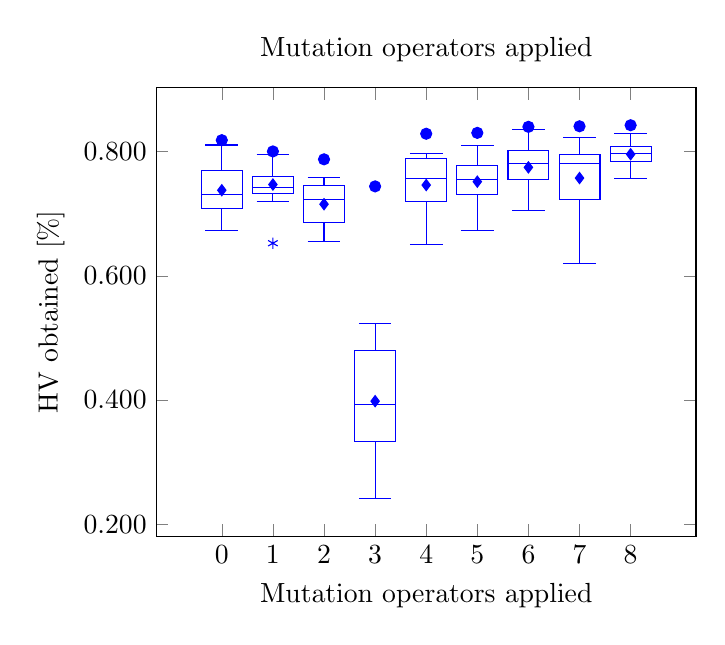
\begin{tikzpicture} 
\begin{axis}[ 
title={Mutation operators applied}, 
boxplot/draw direction=y, 
xtick={1,2,3,4,5,6,7,8,9}, 
xticklabels={0,1,2,3,4,5,6,7,8}, 
x tick label style={rotate=0, align=center}, 
xlabel={Mutation operators applied}, 
y tick label style={/pgf/number format/.cd,fixed,precision=3, zerofill}, 
ylabel={HV obtained [\%]}, 
] 

% ############## Mutations_AMALGAM=0 ################## 
\addplot[boxplot, mark=asterisk, 
boxplot prepared={ 
lower whisker=0.67241, 
upper whisker=0.81075, 
lower quartile=0.70776, 
upper quartile=0.76961, 
median=0.73075, 
average=0.73786}, 
color = blue, solid, area legend] 
coordinates {}; 
\addplot[only marks,mark=*,color = blue]coordinates{(1,0.81844)}; 

% ############## Mutations_AMALGAM=1 ################## 
\addplot[boxplot, mark=asterisk, 
boxplot prepared={ 
lower whisker=0.71918, 
upper whisker=0.79487, 
lower quartile=0.73201, 
upper quartile=0.76059, 
median=0.74231, 
average=0.74704}, 
color = blue, solid, area legend] 
coordinates {
(2,0.6525)}; 
\addplot[only marks,mark=*,color = blue]coordinates{(2,0.80034)}; 

% ############## Mutations_AMALGAM=2 ################## 
\addplot[boxplot, mark=asterisk, 
boxplot prepared={ 
lower whisker=0.65527, 
upper whisker=0.75827, 
lower quartile=0.68519, 
upper quartile=0.74555, 
median=0.72224, 
average=0.71533}, 
color = blue, solid, area legend] 
coordinates {}; 
\addplot[only marks,mark=*,color = blue]coordinates{(3,0.78762)}; 

% ############## Mutations_AMALGAM=3 ################## 
\addplot[boxplot, mark=asterisk, 
boxplot prepared={ 
lower whisker=0.24086, 
upper whisker=0.52265, 
lower quartile=0.33285, 
upper quartile=0.47958, 
median=0.39337, 
average=0.39817}, 
color = blue, solid, area legend] 
coordinates {}; 
\addplot[only marks,mark=*,color = blue]coordinates{(4,0.74405)}; 

% ############## Mutations_AMALGAM=4 ################## 
\addplot[boxplot, mark=asterisk, 
boxplot prepared={ 
lower whisker=0.65105, 
upper whisker=0.79737, 
lower quartile=0.72002, 
upper quartile=0.78931, 
median=0.75737, 
average=0.74617}, 
color = blue, solid, area legend] 
coordinates {}; 
\addplot[only marks,mark=*,color = blue]coordinates{(5,0.82882)}; 

% ############## Mutations_AMALGAM=5 ################## 
\addplot[boxplot, mark=asterisk, 
boxplot prepared={ 
lower whisker=0.67291, 
upper whisker=0.81022, 
lower quartile=0.73129, 
upper quartile=0.7778, 
median=0.75542, 
average=0.7516}, 
color = blue, solid, area legend] 
coordinates {}; 
\addplot[only marks,mark=*,color = blue]coordinates{(6,0.83023)}; 

% ############## Mutations_AMALGAM=6 ################## 
\addplot[boxplot, mark=asterisk, 
boxplot prepared={ 
lower whisker=0.70515, 
upper whisker=0.83585, 
lower quartile=0.7549, 
upper quartile=0.80185, 
median=0.7805, 
average=0.77464}, 
color = blue, solid, area legend] 
coordinates {}; 
\addplot[only marks,mark=*,color = blue]coordinates{(7,0.83995)}; 

% ############## Mutations_AMALGAM=7 ################## 
\addplot[boxplot, mark=asterisk, 
boxplot prepared={ 
lower whisker=0.6204, 
upper whisker=0.82258, 
lower quartile=0.72359, 
upper quartile=0.79503, 
median=0.78095, 
average=0.75746}, 
color = blue, solid, area legend] 
coordinates {}; 
\addplot[only marks,mark=*,color = blue]coordinates{(8,0.84084)}; 

% ############## Mutations_AMALGAM=8 ################## 
\addplot[boxplot, mark=asterisk, 
boxplot prepared={ 
lower whisker=0.75692, 
upper whisker=0.82871, 
lower quartile=0.7835, 
upper quartile=0.80831, 
median=0.79656, 
average=0.79577}, 
color = blue, solid, area legend] 
coordinates {}; 
\addplot[only marks,mark=*,color = blue]coordinates{(9,0.84252)}; 

\end{axis}
\end{tikzpicture}
\end{figure} 

% ######################## UTRP SA Mutation operators applied ######################## 
\begin{figure} 
\centering 
\tikzsetnextfilename{UTRP_DBMOSA_BP_mutation_funcs_AMAL_every_n} 
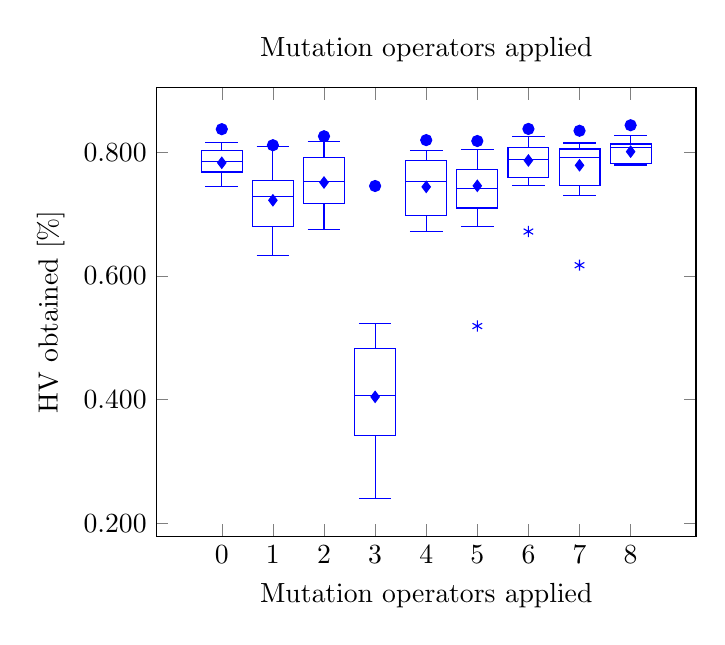
\begin{tikzpicture} 
\begin{axis}[ 
title={Mutation operators applied}, 
boxplot/draw direction=y, 
xtick={1,2,3,4,5,6,7,8,9}, 
xticklabels={0,1,2,3,4,5,6,7,8}, 
x tick label style={rotate=0, align=center}, 
xlabel={Mutation operators applied}, 
y tick label style={/pgf/number format/.cd,fixed,precision=3, zerofill}, 
ylabel={HV obtained [\%]}, 
] 

% ############## Mutations_AMALGAM_every_n=0 ################## 
\addplot[boxplot, mark=asterisk, 
boxplot prepared={ 
lower whisker=0.74458, 
upper whisker=0.81644, 
lower quartile=0.76802, 
upper quartile=0.80227, 
median=0.78569, 
average=0.78297}, 
color = blue, solid, area legend] 
coordinates {}; 
\addplot[only marks,mark=*,color = blue]coordinates{(1,0.83732)}; 

% ############## Mutations_AMALGAM_every_n=1 ################## 
\addplot[boxplot, mark=asterisk, 
boxplot prepared={ 
lower whisker=0.63263, 
upper whisker=0.8095, 
lower quartile=0.67988, 
upper quartile=0.75406, 
median=0.72902, 
average=0.72239}, 
color = blue, solid, area legend] 
coordinates {}; 
\addplot[only marks,mark=*,color = blue]coordinates{(2,0.8114)}; 

% ############## Mutations_AMALGAM_every_n=2 ################## 
\addplot[boxplot, mark=asterisk, 
boxplot prepared={ 
lower whisker=0.67574, 
upper whisker=0.81757, 
lower quartile=0.71662, 
upper quartile=0.79098, 
median=0.75278, 
average=0.75118}, 
color = blue, solid, area legend] 
coordinates {}; 
\addplot[only marks,mark=*,color = blue]coordinates{(3,0.82589)}; 

% ############## Mutations_AMALGAM_every_n=3 ################## 
\addplot[boxplot, mark=asterisk, 
boxplot prepared={ 
lower whisker=0.23991, 
upper whisker=0.52265, 
lower quartile=0.34253, 
upper quartile=0.48244, 
median=0.40733, 
average=0.40471}, 
color = blue, solid, area legend] 
coordinates {}; 
\addplot[only marks,mark=*,color = blue]coordinates{(4,0.74549)}; 

% ############## Mutations_AMALGAM_every_n=4 ################## 
\addplot[boxplot, mark=asterisk, 
boxplot prepared={ 
lower whisker=0.67134, 
upper whisker=0.8031, 
lower quartile=0.6974, 
upper quartile=0.78631, 
median=0.75303, 
average=0.74404}, 
color = blue, solid, area legend] 
coordinates {}; 
\addplot[only marks,mark=*,color = blue]coordinates{(5,0.81966)}; 

% ############## Mutations_AMALGAM_every_n=5 ################## 
\addplot[boxplot, mark=asterisk, 
boxplot prepared={ 
lower whisker=0.67956, 
upper whisker=0.80459, 
lower quartile=0.70988, 
upper quartile=0.77144, 
median=0.74179, 
average=0.74573}, 
color = blue, solid, area legend] 
coordinates {
(6,0.51917)}; 
\addplot[only marks,mark=*,color = blue]coordinates{(6,0.81819)}; 

% ############## Mutations_AMALGAM_every_n=6 ################## 
\addplot[boxplot, mark=asterisk, 
boxplot prepared={ 
lower whisker=0.74649, 
upper whisker=0.82563, 
lower quartile=0.75992, 
upper quartile=0.80781, 
median=0.78768, 
average=0.78674}, 
color = blue, solid, area legend] 
coordinates {
(7,0.67189)}; 
\addplot[only marks,mark=*,color = blue]coordinates{(7,0.83773)}; 

% ############## Mutations_AMALGAM_every_n=7 ################## 
\addplot[boxplot, mark=asterisk, 
boxplot prepared={ 
lower whisker=0.72969, 
upper whisker=0.81491, 
lower quartile=0.74656, 
upper quartile=0.80519, 
median=0.79102, 
average=0.77898}, 
color = blue, solid, area legend] 
coordinates {
(8,0.61748)}; 
\addplot[only marks,mark=*,color = blue]coordinates{(8,0.83474)}; 

% ############## Mutations_AMALGAM_every_n=8 ################## 
\addplot[boxplot, mark=asterisk, 
boxplot prepared={ 
lower whisker=0.77947, 
upper whisker=0.82736, 
lower quartile=0.78228, 
upper quartile=0.81334, 
median=0.80771, 
average=0.80101}, 
color = blue, solid, area legend] 
coordinates {}; 
\addplot[only marks,mark=*,color = blue]coordinates{(9,0.84368)}; 

\end{axis}
\end{tikzpicture}
\end{figure} 

% ######################## UTRP SA Mutation operators applied ######################## 
\begin{figure} 
\centering 
\tikzsetnextfilename{UTRP_DBMOSA_BP_mutation_funcs_Counts_normal} 
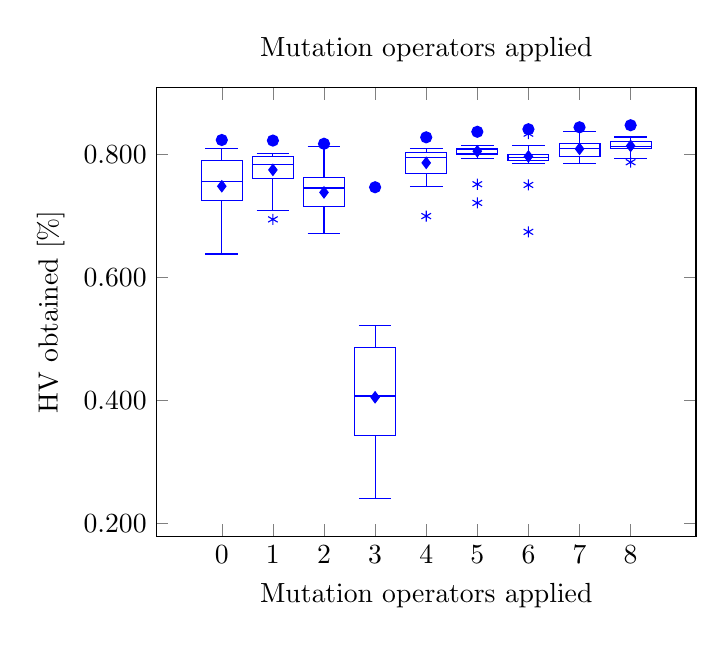
\begin{tikzpicture} 
\begin{axis}[ 
title={Mutation operators applied}, 
boxplot/draw direction=y, 
xtick={1,2,3,4,5,6,7,8,9}, 
xticklabels={0,1,2,3,4,5,6,7,8}, 
x tick label style={rotate=0, align=center}, 
xlabel={Mutation operators applied}, 
y tick label style={/pgf/number format/.cd,fixed,precision=3, zerofill}, 
ylabel={HV obtained [\%]}, 
] 

% ############## Mutations_Counts_normal=0 ################## 
\addplot[boxplot, mark=asterisk, 
boxplot prepared={ 
lower whisker=0.63823, 
upper whisker=0.80967, 
lower quartile=0.72569, 
upper quartile=0.79016, 
median=0.75579, 
average=0.7484}, 
color = blue, solid, area legend] 
coordinates {}; 
\addplot[only marks,mark=*,color = blue]coordinates{(1,0.82363)}; 

% ############## Mutations_Counts_normal=1 ################## 
\addplot[boxplot, mark=asterisk, 
boxplot prepared={ 
lower whisker=0.70887, 
upper whisker=0.80111, 
lower quartile=0.7609, 
upper quartile=0.7968, 
median=0.7832, 
average=0.77508}, 
color = blue, solid, area legend] 
coordinates {
(2,0.69457)}; 
\addplot[only marks,mark=*,color = blue]coordinates{(2,0.82269)}; 

% ############## Mutations_Counts_normal=2 ################## 
\addplot[boxplot, mark=asterisk, 
boxplot prepared={ 
lower whisker=0.67179, 
upper whisker=0.81236, 
lower quartile=0.71523, 
upper quartile=0.76255, 
median=0.7455, 
average=0.73836}, 
color = blue, solid, area legend] 
coordinates {}; 
\addplot[only marks,mark=*,color = blue]coordinates{(3,0.8175)}; 

% ############## Mutations_Counts_normal=3 ################## 
\addplot[boxplot, mark=asterisk, 
boxplot prepared={ 
lower whisker=0.24015, 
upper whisker=0.52265, 
lower quartile=0.34319, 
upper quartile=0.48589, 
median=0.40733, 
average=0.40528}, 
color = blue, solid, area legend] 
coordinates {}; 
\addplot[only marks,mark=*,color = blue]coordinates{(4,0.7468)}; 

% ############## Mutations_Counts_normal=4 ################## 
\addplot[boxplot, mark=asterisk, 
boxplot prepared={ 
lower whisker=0.74761, 
upper whisker=0.80916, 
lower quartile=0.76949, 
upper quartile=0.80388, 
median=0.79545, 
average=0.78648}, 
color = blue, solid, area legend] 
coordinates {
(5,0.69994)}; 
\addplot[only marks,mark=*,color = blue]coordinates{(5,0.82798)}; 

% ############## Mutations_Counts_normal=5 ################## 
\addplot[boxplot, mark=asterisk, 
boxplot prepared={ 
lower whisker=0.7941, 
upper whisker=0.81461, 
lower quartile=0.80094, 
upper quartile=0.80974, 
median=0.80745, 
average=0.80531}, 
color = blue, solid, area legend] 
coordinates {
(6,0.72137)
(6,0.75171)}; 
\addplot[only marks,mark=*,color = blue]coordinates{(6,0.83698)}; 

% ############## Mutations_Counts_normal=6 ################## 
\addplot[boxplot, mark=asterisk, 
boxplot prepared={ 
lower whisker=0.78568, 
upper whisker=0.81487, 
lower quartile=0.79065, 
upper quartile=0.80073, 
median=0.79513, 
average=0.79692}, 
color = blue, solid, area legend] 
coordinates {
(7,0.75058)
(7,0.83387)
(7,0.67426)}; 
\addplot[only marks,mark=*,color = blue]coordinates{(7,0.84115)}; 

% ############## Mutations_Counts_normal=7 ################## 
\addplot[boxplot, mark=asterisk, 
boxplot prepared={ 
lower whisker=0.78547, 
upper whisker=0.83815, 
lower quartile=0.79673, 
upper quartile=0.81736, 
median=0.81022, 
average=0.8092}, 
color = blue, solid, area legend] 
coordinates {}; 
\addplot[only marks,mark=*,color = blue]coordinates{(8,0.84429)}; 

% ############## Mutations_Counts_normal=8 ################## 
\addplot[boxplot, mark=asterisk, 
boxplot prepared={ 
lower whisker=0.79334, 
upper whisker=0.82857, 
lower quartile=0.80917, 
upper quartile=0.82112, 
median=0.8132, 
average=0.81402}, 
color = blue, solid, area legend] 
coordinates {
(9,0.7875)}; 
\addplot[only marks,mark=*,color = blue]coordinates{(9,0.84763)}; 

\end{axis}
\end{tikzpicture}
\end{figure} 
\begin{table}
\centering
\caption{Legend for the boxplot.}
\begin{tabular}{ll}
\toprule
 Index &                                               Name \\
\midrule
     0 &               [MSC\_add\_terminal, MSC\_del\_terminal] \\
     1 &                        [Add\_vertex, Delete\_vertex] \\
     2 &       [Trim\_one\_terminal\_cb, Grow\_one\_terminal\_cb] \\
     3 &       [Insert\_inside\_vertex, Delete\_inside\_vertex] \\
     4 & [Add\_vertex, Delete\_vertex, Insert\_inside\_verte... \\
     5 &        [Add\_vertex, Delete\_vertex, Intertwine\_two] \\
     6 & [Add\_vertex, Delete\_vertex, Insert\_inside\_verte... \\
     7 & [MSC\_add\_terminal, MSC\_del\_terminal, Insert\_ins... \\
     8 & [Add\_vertex, Delete\_vertex, Insert\_inside\_verte... \\
\bottomrule
\end{tabular}
\end{table}

\end{document}
